\documentclass{article}
\usepackage{arxiv}

\usepackage[utf8]{inputenc}
\usepackage[english]{babel}
\usepackage[T1]{fontenc}
\usepackage{url}
\usepackage{booktabs}
\usepackage{amsfonts}
\usepackage{amssymb}
\usepackage{nicefrac}
\usepackage{hyperref}
\usepackage{microtype}
\usepackage{lipsum}
\usepackage{graphicx}
\usepackage{natbib}
\usepackage{doi}
\usepackage[colorinlistoftodos]{todonotes}
\usepackage{hyperref}

\renewcommand{\headeright}{Draft}
\renewcommand{\undertitle}{Draft}
\newcommand{\Hquad}{\hspace{0.5em}} 

\title{Detection of machine-generated fragments in text}

\author{ Anastasiya Voznyuk \\
	Department of Applied Informatics and Mathematics\\
	Moscow Institute of Physics and Technology\\
	\texttt{vozniuk.ae@phystech.edu} \\
	%\texttt{\href{https://colab.research.google.com/drive/1HBB8002s5_tFgFxGzIZQcBmsOsW6YcMh?usp=sharing} {Project code}} \\
    \\
    \textbf{Andrey Grabovoy} \\
	Moscow Institute of Physics and Technology\\
    Antiplagiat Company \\
	%% Address \\
	\texttt{grabovoy@ap-team.ru}}
	%% \And
	%% Coauthor \\
	%% Affiliation \\
	%% Address \\
	%% \texttt{email} \\
	%% \And
	%% Coauthor \\
	%% Affiliation \\
	%% Address \\
	%% \texttt{email} \\

\date{}

\renewcommand{\shorttitle}{Detection of machine-generated fragments in text}

%%% Add PDF metadata to help others organize their library
%%% Once the PDF is generated, you can check the metadata with
%%% $ pdfinfo template.pdf
\hypersetup{
pdftitle={A template for the arxiv style},
pdfsubject={q-bio.NC, q-bio.QM},
pdfauthor={Voznyuk Anastasiya},
pdfkeywords={Detection},
}

\begin{document}
\maketitle

\begin{abstract}
	This paper considers the problem of detecting machine-generated parts of text in the document. We introduce a model, that can detect such text fragments and distinguish their origin among several language models. To solve this problem we combine two models. The objective of the first one is to divide document into fragments of human-written text and machine-generated text. The second model aims to classify the generated fragments according to the language model from which they were obtained. In the computational experiment, we analyse the quality of such approach on dataset of documents with fragments generated by GPT-2 and GPT-3.
\end{abstract}


\keywords{Text Generation, Detection of Machine-generated text, Neural Authorship Attribution, Machine Learning, Natural Language Processing}

\section{Introduction}

% \cite{EVL:1}
In recent years there has been a rapid development of language models for text generation, transformers in particular, for example GPT\cite{gpt}, GPT-2\cite{gpt2}, GPT-3\cite{gpt3}, CTRL\cite{ctrl} and mT5\cite{mt5}. Problem of detecting machine-generated text has become more relevant recently due to the released ChatGPT model by OpenAI. This model was learnt on massive amounts of data and now is able to provide texts that are hardly distinguishable from human texts. The opposite task of detecting machine-generated text becomes more important due to many possible malicious usages of this technology. One can analyse the whole text or fragments of text.
We will focus on methods of subtracting the text-generated fragments in the set of documents.\\
With increased computational resources past statistical methods were applied to the novel detection problem. One of them was prediction entropy as an indicator of fake text, as described in \cite{relativeentropy}. Also perplexity\cite{perplexity} of the text or frequency of rare bigrams \cite{rare_bigrams} or value of tf-idf \cite{solaiman} can be taken into account. Another approach is to use classifiers that try to label given texts \cite{Kuznetsov}.\\
For a long period recursive neural networks like LSTM were showing best results at solving the problem of detection. At 2018 the mechanism of self-attention\cite{Vaswani} was introduced and transformers have become new state-of-the-art approach.  Every new model has its own features and is usually learnt on larger amounts of data, but attention mechanism always stays. These model can be used in detection of machine-generated text in two ways\cite{solaiman}. The first method is using a language model that searches for artefacts from  methods, which most models are using for generating concise texts \cite{gltr}. Additional training on new data is not required. The second method is fine-tuning based detection: one fine-tunes a language model to “detect itself” with using some stochastic methods, for example top-k, top-p sampling etc.\\
The first step is to divide each document into non-overlapping blocks of sentences. We take the baseline from work\cite{Kuznetsov} on plagiarism detection. Also metrics and construction of loss function from the works about text segmentation problem can be borrowed. We suppose, that within a fragment with artificial text there is a finished idea and similar semantic structure. For example, loss function is described at \cite{ts_loss}, and metrics are described at \cite{ts_metrics}. The next step is to detect the origin of machine-generated text and this can be done with usage of transformer-based models. This papers presents computational experiments with these models to combine them in one model and analyse the parameters on which the best performance will be obtained. Dataset will be constructed from existing datasets, such as GPT-2 output dataset\cite{gpt2-dataset} and RUaTD competition dataset\cite{ruatd-dataset}.  %%%%---!!
\section{Problem statement}

Let $\mathbf{W}$ be our alphabet, tokens consists from characters from that alphabet.

Let $$\mathbb{D} = \Bigl\{\Big[t_j\Big]_{j=1}^n \Hquad|\Hquad t_j \in \mathbf{W}, n \in \mathbb{N}\Bigr\}$$ be the space of our documents.

We have set of $n$ documents
$$\mathbf{D} = \bigcup_{i=1}^{n}D^i, D^i \in \mathbb{D}$$

%Each document  $D^i$ consists of $d_i$ tokens $t_1^i, t_2^i, ..., t_{d_i}^i$, where $t_j^i \in \mathbf{W}$ .
We have $K$ classes of our text-generative models, that generated fragments of text in $\mathbf{D}$.

We have $K + 1$ labels, that we will use for multiclass classification, where $0$ - label of human-written fragment, ${1...K}$ - labels that represent corresponding language model, let $\mathbf{C}$ be our set of labels.

Our model $\mathbf{\phi}$ is a superposition of two mappings, $\mathbf{f}$ and $\mathbf{g}$. Mapping $\mathbf{f}$ is responsible for text segmentation. Mapping $\mathbf{g}$ is responsible for classifying obtained fragments.

$$\mathbf{\phi} : \mathbf{g} \circ \mathbf{f}$$


$$\mathbf{\phi}: \mathbb{D} \rightarrow \mathbb{T} \qquad \mathbb{T} = \Bigl\{\Big[t_{s_j}, t_{f_j}, C_j\Big]_{j = 1}^{J} \Hquad|\Hquad t_{s_j} = t_{f_{j - 1}},\Hquad s_j \in \mathbb{N}_0,\Hquad f_j \in \mathbb{N}, \Hquad C_j \in \mathbf{C}\Bigr\},$$

where $J$ - number of fragments in segmentation of the document, $t_{s_j}$ - starting index of the $j$-th fragment,  $t_{f_j}$ - finishing index of the $j$-th fragment,  $C_{j}$ - class of the $j$-th fragment.



\subsection{Text fragmentation}
The first step is to divide our text into fragments of different origin.

$$\mathbf{f}: \mathbb{D} \rightarrow \mathbf{T}^* \qquad \mathbf{T}^* = \Bigl\{\Big[t_{s_j}, t_{f_j}\Big]_{j = 1}^{J}\quad|\quad t_{s_j} = t_{f_{j - 1}}, s_j \in \mathbb{N}_0, f_j \in \mathbb{N}\Bigr\},$$

where $s_j$ - start of the $j$-th fragment and $f_j$ - end of the $j$-th fragment.

Thus, $\mathbf{T}^*$ is a set of all possible sequences of non-overlapping blocks of texts, that covers complete document.

We assume that in each document blocks of text with the same origin is big enough. Thus, we search for style changes on sentence levels. Style change indicates that several next sentences staring from the beginning of the style change have different origin. Each sentence receive a label $0$ or $1$, where 0 means it is a human-written sentence and 1 is a machine-generated sentence. A fragment is a sequence of neighbouring sentences of maximum possible length, that have the same label. We repeat this process for every document in given set of document. 

Each document segments have to be clustered into $c$ clusters, where $c$  =  $|\textbf{C}|$. 

\subsection{Fragment classification}

The second step is to classify each fragment with label from $\mathbf{C}$.
$$\mathbf{g}: \mathbf{T}^* \rightarrow \mathbf{C}$$

We apply that function to every text fragment, obtained from the previous step. This is a classical multi-classification task. We will use cross-entropy as a loss function:

$$\mathbf{Loss_{cls}}(x) = \sum_{i=0}^K-p(x)\log q(x)$$ 
where $p(x)$ - probability of object $x$ to be actually labelled with $i$,
$q(x)$ -  probability of object $x$ to be labelled with $i$  in prediction.

\subsection{Metrics}

To measure how good our model is capable to divide our into fragments we will use BCubed\cite{bcubed} measurements.
Let $S$ be our true segmentation and $\hat{S}$  is the predicted segmentation. We divide the segments from the true segmentation $S$ and the predicted segmentation $\hat{S}$ each into sets of segments $S_i$, $i\in\{1..c\}$, and $\hat{S}_j$, $j\in\{1..\hat{c}\}$, where $c$ is the true number of authors, and $\hat{c}$ the predicted number of authors. Let $l$ be a function that maps a segment to its length. If $S$ is a set of segment, $l(S) = \sum_{s \in S}l(s)$. BCubed precision of an item is the proportion of items in its cluster which have the item’s label, including itself. In our tasks item is a segment from a document, extracted by model. The overall BCubed precision is the averaged precision of all items in the distribution.  

 $$ P_{\mathrm{B}^3} = \sum_{i=1}^c \frac{1}{l(S_i)}\sum_{j=1}^{\hat{c}}
	\sum_{s\in S_i}	\sum_{\hat{s}\in\hat{S}_j} l(s\cap \hat{s})^2, $$
$$ R_{\mathrm{B}^3} = \sum_{j=1}^{\hat{c}} \frac{1}{l(\hat{S}_j)}\sum_{i=1}^{c}
	\sum_{s\in S_i}	\sum_{\hat{s}\in\hat{S}_j} l(s\cap \hat{s})^2, $$

Also, we would like to measure whether our model detects a segment of different origin as a whole or in several segments. Let it be a granularity\cite{granularity} of model:

$$gran(S, R) = \frac{1}{|S_{R}|}\sum_{s \in S_{R}}|R_{S}|,$$

where $S_{R} \subseteq S$ - cases of proved chmage of author in $R$, and $R_{S} \subseteq R$ are detections -alleged changes of author in $s$.

\section{Computational Experiment}

The goal of computational experiment is to analyse how good baseline solution in classifying fragments of text. RUATD  competition, which provided the dataset, also provided accuracy score for their baseline solutions. One solutuion uses tf-idf + logistic regression approach, the other solution uses fine-tuned BERT. We will use the second approach, but our own solution and compare our results with the ones, suggested by the authours of competition.
% The task is to find the optimal parameters of our model in which certain requirements on the quality of the model will be achieved.
% For text fragmentation we use Gradient Boosting Regression Tree for classifying the sentences, as described in \cite{Kuznetsov}. The optimal parameters are (???).
% %(n_estimators=200, max_depth=4)%
% %by maximization of the Area-Under-Curve classification measure.
% Also we detect outliers: if a sentence is label-classified with some value higher than threshold, we will label it as a machine generated sentence.

% For fragment classification we suggest to use an approach, described in \cite{gritsay2022}, namely RoBERTa-base model for English texts and XLM-RoBERTa-base model for Russian texts.

\subsection{Dataset}

To test how good our model in text segmentation we generate a dataset of 10000 documents, each of documents consists of 5-6 fragments of different origin. Human-written fragments were taken from Wikipedia Dataset \footnote{\url{https://huggingface.co/datasets/wikipedia}}. Machine-generated texts were generated by Sberbank-AI model\footnote{\url{https://huggingface.co/sberbank-ai/rugpt3small_based_on_gpt2}}. \\
For our experiment with classification we took the data, that was collected for RUATD 2022 competition\cite{ruatd-dataset} for multitask classification. The test dataset contains 215105 short fragments, that were generated by different 13 models. Authors claim that various language models fine-tuned on different tasks: machine translation, paraphrasing, summarization, simplification and unconditional text generation - were used to generate texts. Moreover, the part of the set was annotated automatically by different generative models. Among models there are several versions of ruGPT, mT5 and ruT5 and M-BART.

\subsection{Configuration of algorithm run}

We used only a part of dataset for the sake of decreasing the time of training. 

Our pipeline for extracting segments from the document consists of tokenization of sentences, basic feature extraction, feature transofrmation and clustering. 

Feature extraction was conducted with a sliding window, that includes context of each token. The size of sliding window was 120 tokens. Among features, that were extracted, were stop words counts, Bag of Words, chracter tri-gram counts. After that we tranformed these features with linear layer. For optimization of this step we used RMSProp. On Figure 3 one can see the loss over sample size during training. Clustering was done with k-means.


For tokenization of sentences in text fragments we used pretrained embedding from \texttt{bert-base-multilingual-cased}\footnote{\url{https://github.com/google-research/bert/blob/master/multilingual.md}}. The same model was fine-tuned for our sequence classification task. We trained our model for 3 epochs. For optimization we used AdamW optimization algorithm\cite{adam-w}.


\subsection{List of expected figures and tables}
\begin{enumerate}
    \item Table of train accuracy and validation accuracy on each epoch
    \item Graph of validation / train loss versus epoch - Figure 1
    \item Graph of Precision-Recall Curve for every class - Figure 2
\end{enumerate}

% The dataset, PAN-PC-11\cite{pan-dataset} was intended to use for intrinsic plagiarism detection. We will analyse our task on sentence-level, this will be out tokens. The test collection consists of 4753 documents and is split into 10 folds. Each folds contains 500 documents except for the smaller fold 10. We used it as a benchmark for measuring, how good our model is in fragmenting a document.

% The dataset, used for text classification problem was GPT-2 output dataset\cite{gpt2-dataset}, which allows  to compare data from models with different numbers of parameters and different sampling methods. 

% For evaluating our task we will need to generate our own dataset with document by taking fragments from this dataset and from RUaTD task dataset \cite{ruatd-dataset} and combining them with fragments of human-written text. However, one should be careful when generating a document, we need to pay attention and do not let our generator to take fragments from different domains. 


  
\section{Preliminary report}

We received 56$\%$ of accuracy with 3 epoch of training only using the part of the dataset. It is les than the score, provided by the authors of competition, which is 59$\%$, but this difference is explained by smaller size of the dataset. Also we may suggest that due to increasing loss on validation set, our model started to overfit. Another issue with the quality of classification on some classes: for some classes there's a small recall, e.g class 6. For some classes there's both small recall and small precision, e.g class 3, class 12 and class 13. For some of class it is happened because of small amount of these classes in dataset. 


\begin{table}[bhtp]
	\centering
	\caption{Table of train accuracy and validation accuracy on each epoch}
	\label{tbl:space_and_subspace}
	\begin{tabular}{| c | c | c | c | }
		\hline
		Number of epoch & Train. loss & Valid.loss & Valid. accuracy \\
		\hline
		1 & 1.30  & 1.26 & 0.54  \\
        \hline
		2 & 1.07 & 1.27 & 0.56  \\
		\hline
        3 & 0.86  & 1.35 & 0.56  \\
        \hline
	\end{tabular}
\end{table}

\begin{figure}[bhtp]
	\includegraphics[width=\textwidth]{Unknown-2.png}
	\caption{Graph of validation / train loss versus epoch}
	\label{fig:1}
\end{figure}


\begin{figure}[bhtp]
	\includegraphics[width=\textwidth]{Unknown.png}
	\caption{Graph of Precision-Recall Curve for every class}
	\label{fig:2}
\end{figure}


\begin{figure}[bhtp]
	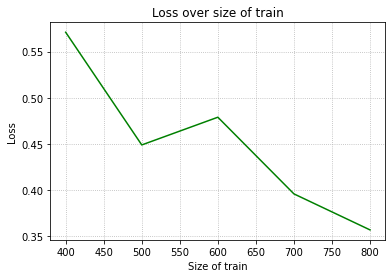
\includegraphics[width=\textwidth]{loss.png}
	\caption{Graph on Loss Function}
	\label{fig:3}
\end{figure}



\bibliographystyle{plain}
\bibliography{references}

\end{document}